% Options for packages loaded elsewhere
\PassOptionsToPackage{unicode}{hyperref}
\PassOptionsToPackage{hyphens}{url}
\PassOptionsToPackage{dvipsnames,svgnames,x11names}{xcolor}
%
\documentclass[
  a4paper,
]{article}

\usepackage{amsmath,amssymb}
\usepackage{iftex}
\ifPDFTeX
  \usepackage[T1]{fontenc}
  \usepackage[utf8]{inputenc}
  \usepackage{textcomp} % provide euro and other symbols
\else % if luatex or xetex
  \usepackage{unicode-math}
  \defaultfontfeatures{Scale=MatchLowercase}
  \defaultfontfeatures[\rmfamily]{Ligatures=TeX,Scale=1}
\fi
\usepackage{lmodern}
\ifPDFTeX\else  
    % xetex/luatex font selection
\fi
% Use upquote if available, for straight quotes in verbatim environments
\IfFileExists{upquote.sty}{\usepackage{upquote}}{}
\IfFileExists{microtype.sty}{% use microtype if available
  \usepackage[]{microtype}
  \UseMicrotypeSet[protrusion]{basicmath} % disable protrusion for tt fonts
}{}
\makeatletter
\@ifundefined{KOMAClassName}{% if non-KOMA class
  \IfFileExists{parskip.sty}{%
    \usepackage{parskip}
  }{% else
    \setlength{\parindent}{0pt}
    \setlength{\parskip}{6pt plus 2pt minus 1pt}}
}{% if KOMA class
  \KOMAoptions{parskip=half}}
\makeatother
\usepackage{xcolor}
\usepackage[top=2.54cm,right=2.54cm,bottom=2.54cm,left=2.54cm]{geometry}
\setlength{\emergencystretch}{3em} % prevent overfull lines
\setcounter{secnumdepth}{-\maxdimen} % remove section numbering
% Make \paragraph and \subparagraph free-standing
\makeatletter
\ifx\paragraph\undefined\else
  \let\oldparagraph\paragraph
  \renewcommand{\paragraph}{
    \@ifstar
      \xxxParagraphStar
      \xxxParagraphNoStar
  }
  \newcommand{\xxxParagraphStar}[1]{\oldparagraph*{#1}\mbox{}}
  \newcommand{\xxxParagraphNoStar}[1]{\oldparagraph{#1}\mbox{}}
\fi
\ifx\subparagraph\undefined\else
  \let\oldsubparagraph\subparagraph
  \renewcommand{\subparagraph}{
    \@ifstar
      \xxxSubParagraphStar
      \xxxSubParagraphNoStar
  }
  \newcommand{\xxxSubParagraphStar}[1]{\oldsubparagraph*{#1}\mbox{}}
  \newcommand{\xxxSubParagraphNoStar}[1]{\oldsubparagraph{#1}\mbox{}}
\fi
\makeatother


\providecommand{\tightlist}{%
  \setlength{\itemsep}{0pt}\setlength{\parskip}{0pt}}\usepackage{longtable,booktabs,array}
\usepackage{calc} % for calculating minipage widths
% Correct order of tables after \paragraph or \subparagraph
\usepackage{etoolbox}
\makeatletter
\patchcmd\longtable{\par}{\if@noskipsec\mbox{}\fi\par}{}{}
\makeatother
% Allow footnotes in longtable head/foot
\IfFileExists{footnotehyper.sty}{\usepackage{footnotehyper}}{\usepackage{footnote}}
\makesavenoteenv{longtable}
\usepackage{graphicx}
\makeatletter
\def\maxwidth{\ifdim\Gin@nat@width>\linewidth\linewidth\else\Gin@nat@width\fi}
\def\maxheight{\ifdim\Gin@nat@height>\textheight\textheight\else\Gin@nat@height\fi}
\makeatother
% Scale images if necessary, so that they will not overflow the page
% margins by default, and it is still possible to overwrite the defaults
% using explicit options in \includegraphics[width, height, ...]{}
\setkeys{Gin}{width=\maxwidth,height=\maxheight,keepaspectratio}
% Set default figure placement to htbp
\makeatletter
\def\fps@figure{htbp}
\makeatother

% Preámbulo
\usepackage{comment} % Permite comentar secciones del código
\usepackage{marvosym} % Agrega símbolos adicionales
\usepackage{graphicx} % Permite insertar imágenes
\usepackage{mathptmx} % Fuente de texto matemática
\usepackage{amssymb} % Símbolos adicionales de matemáticas
\usepackage{lipsum} % Crea texto aleatorio
\usepackage{amsthm} % Teoremas y entornos de demostración
\usepackage{float} % Control de posiciones de figuras y tablas
\usepackage{rotating} % Rotación de elementos
\usepackage{multirow} % Celdas combinadas en tablas
\usepackage{tabularx} % Tablas con ancho de columna ajustable
\usepackage{mdframed} % Marcos alrededor de elementos flotantes

% Series de tiempo
\usepackage{booktabs}


% Configuración adicional

\makeatletter
\@ifpackageloaded{caption}{}{\usepackage{caption}}
\AtBeginDocument{%
\ifdefined\contentsname
  \renewcommand*\contentsname{Tabla de contenidos}
\else
  \newcommand\contentsname{Tabla de contenidos}
\fi
\ifdefined\listfigurename
  \renewcommand*\listfigurename{Listado de Figuras}
\else
  \newcommand\listfigurename{Listado de Figuras}
\fi
\ifdefined\listtablename
  \renewcommand*\listtablename{Listado de Tablas}
\else
  \newcommand\listtablename{Listado de Tablas}
\fi
\ifdefined\figurename
  \renewcommand*\figurename{Figura}
\else
  \newcommand\figurename{Figura}
\fi
\ifdefined\tablename
  \renewcommand*\tablename{Tabla}
\else
  \newcommand\tablename{Tabla}
\fi
}
\@ifpackageloaded{float}{}{\usepackage{float}}
\floatstyle{ruled}
\@ifundefined{c@chapter}{\newfloat{codelisting}{h}{lop}}{\newfloat{codelisting}{h}{lop}[chapter]}
\floatname{codelisting}{Listado}
\newcommand*\listoflistings{\listof{codelisting}{Listado de Listados}}
\makeatother
\makeatletter
\makeatother
\makeatletter
\@ifpackageloaded{caption}{}{\usepackage{caption}}
\@ifpackageloaded{subcaption}{}{\usepackage{subcaption}}
\makeatother
\ifLuaTeX
\usepackage[bidi=basic]{babel}
\else
\usepackage[bidi=default]{babel}
\fi
\babelprovide[main,import]{spanish}
% get rid of language-specific shorthands (see #6817):
\let\LanguageShortHands\languageshorthands
\def\languageshorthands#1{}
\ifLuaTeX
  \usepackage{selnolig}  % disable illegal ligatures
\fi
\usepackage[]{biblatex}
\addbibresource{../../../references.bib}
\usepackage{bookmark}

\IfFileExists{xurl.sty}{\usepackage{xurl}}{} % add URL line breaks if available
\urlstyle{same} % disable monospaced font for URLs
\hypersetup{
  pdftitle={Notas de Clase Series de Tiempo},
  pdfauthor={Edison Achalma},
  pdflang={es},
  colorlinks=true,
  linkcolor={blue},
  filecolor={Maroon},
  citecolor={Blue},
  urlcolor={Blue},
  pdfcreator={LaTeX via pandoc}}

\title{Notas de Clase Series de Tiempo}
\usepackage{etoolbox}
\makeatletter
\providecommand{\subtitle}[1]{% add subtitle to \maketitle
  \apptocmd{\@title}{\par {\large #1 \par}}{}{}
}
\makeatother
\subtitle{Descubre cómo seleccionar hardware, descargar la imagen ISO y
preparar los medios de instalación. Exploraremos opciones para probar o
instalar Linux en tu equipo.}
\author{Edison Achalma}
\date{2023-08-27}

\begin{document}
\maketitle

\section{Procesos Basados en Vectores
Autoregresivos}\label{procesos-basados-en-vectores-autoregresivos}

\chapter{Procesos basados en Vectores Autoregresivos}

En este capítulo romperemos el supuesto de que el análisis es
univariado, ya que introduciremos la posibilidad de que los procesos
generadores de datos compartan información entre dos o más series. Como
primer aproximación desarrollaremos el concepto de Causalidad de
Granger. Mediante esta metodología discutiremos cuando dos series se
causan estadísticamente. Posteriormente, introduciremos una técnica más
sofisticada conocida como la metodología de Vectores Autoregresivos
(VAR), la cual es una generalización de los procesos AR que analizamos
al principio del curso.

\subsection{Causalidad de Granger}\label{causalidad-de-granger}

Hasta ahora hemos supuesto que una serie puede ser explicada únicamente
con la información contenida en ella misma. No obstante, en adelante
trataremos de analizar el caso en el que buscamos determinar relaciones
entre variables y cómo el comportamiento de una serie influye en las
demás. Algunas relaciones más importantes son las llamadas causalidad.
En este caso analizaremos el procedimiento de Granger (1969), conocido
como causalidad de Granger. En adelante asumiremos que las series
involucradas son debílmente estacionarias.

Sean \(X\) y \(Y\) dos series debílmente estacionarias. Definamos a
\(I_t\) un conjunto de toda la información disponible hasta el momento
\(t\). Asimismo, digamos que \(\overline{X}_t\) y \(\overline{Y}_t\) son
los conjuntos de toda la información disponible (actual y pasada) de
\(X\) y \(Y\), respectivamente. Es decir: \begin{eqnarray}
    \overline{X}_t & := & \{ X_t, X_{t-1}, X_{t-2}, \ldots \} \\
    \overline{Y}_t & := & \{ Y_t, Y_{t-1}, Y_{t-2}, \ldots \} \\
    I_t & := & \overline{X}_t + \overline{Y}_t
\end{eqnarray}

Adicionalmnete, definamos \(\sigma^2(.)\) como la varianza del término
de error estimado de una regresión dada. Dicho lo anterior, decimos que:

\begin{enumerate}
    \item Existe Causalidad de Granger o $X$ causa a $Y$ si y solo si, una regresión lineal da como resultado que: 
    $$
        \sigma^2 (Y_{t+1} | I_t) < \sigma^2 (Y_{t+1} | I_t - X_t)    
    $$
    
    Es decir, que la variabilidad del término de error de una regresión lineal de $Y$ sobre el conjunto de toda la información aplicada a un pronóstico de $Y_{t+1}$ es MENOR que la variabilidad del término de error de una regresión lineal de $Y$ sobre el conjunto de la información de $Y$ aplicada a un pronóstico de $Y_{t+1}$.
    
    \item Existe Causalidad de Granger Instantanéa $X$ causa de forma instantanéa a $Y$ si y solo si, una regresión lineal da como resultado:
    $$
        \sigma^2 (Y_{t+1} | \{ I_t, X_{t+1} \}) < \sigma^2 (Y_{t+1} | I_t)
    $$
    
\end{enumerate}

La definción anterior aplica de igual forma si se reemplaza a \(X\) por
\(Y\) y a \(Y\) por \(X\), respectivamente. De acuerdo a la definición
anterior, existen 5 diferentes posibilidades de relaciones causales
entre las dos series:

\begin{enumerate}
\item $X$ y $Y$ son independientes: $(X, Y)$;

\item Existe solo causalidad instantanéa: $(X - Y)$;

\item $X$ causa a $Y$: $(X \longrightarrow Y)$;

\item $Y$ causa a $X$: $(X \longleftarrow Y)$, y

\item Ambas series se causan: $(X \longleftrightarrow Y)$.

\end{enumerate}

Por lo anterior, representaremos mediante una \(AR(p)\) con variables
exógenas lo siguiente: \[
    A(L) 
    \begin{bmatrix}
    Y_t \\ X_t
    \end{bmatrix}
    =
    \begin{bmatrix}
    a_{11}(L) & a_{12}(L) \\ a_{21}(L) & a_{22}(L)
    \end{bmatrix}
    \begin{bmatrix}
    Y_t \\ X_t
    \end{bmatrix}
    =
    \begin{bmatrix}
    V_t \\ U_t
    \end{bmatrix}
    \label{Granger_Eq}
\]

O en su versión \(MA(q)\) con variables exógenas: \[
    \begin{bmatrix}
    Y_t \\ X_t
    \end{bmatrix}
    =
    B(L)
    \begin{bmatrix}
    V_t \\ U_t
    \end{bmatrix}
    =
    \begin{bmatrix}
    b_{11}(L) & b_{12}(L) \\ b_{21}(L) & b_{22}(L)
    \end{bmatrix}
    \begin{bmatrix}
    V_t \\ U_t
    \end{bmatrix}
\]

Para determinar el test de causalidad utilizaremos una especificación
similar a la de la ecuación (\ref{Granger_Eq}). Para probar si \(X\)
causa a \(Y\) consideraremos la siguiente regresión: \[
    Y_t = \alpha_0 + \sum^{k_1}_{k = 1} a^k_{11} Y_{t-k} + \sum^{k_2}_{k = k_0} a^k_{12} X_{t-k} + U_{1,t}
\]

Donde \(k_0 = 1\) y, en general, se asume que \(k_1 = k_2\). Asimismo,
el valor de estas constantes se puede determinar con el cirterio de
Akaike (o cualquier otro criterio de información). No obstante, algunos
autores sugieren que una buena práctica es considerar valores de \(k_1\)
y \(k_2\) 4, 8, 12 y 16.

Dicho lo anterior, el test de causalidad de Granger se establece con una
prueba F (similar a la definiada en el Apéndice de estas notas), en la
cual se prueba la siguiente hipótesis nula: \[
    H_0: a^1_{12} = a^2_{12} = \ldots = a^{k2}_{12} = 0
\]

Ahora veámos un ejemplo. Consideremos como variables analizadas al
Índice Nacional de Precios al Consumidor (\(INPC_t\)), al Tipo de Cambio
(\(TDC_t\)) y al rendimiento anual de los Cetes a 28 días
(\(CETE28_t\)), todas desestacionalizadas para el periodo de enero de
2000 a julio de 2019. Dado que la metodología de Granger supone que las
series son estacionarias, utilizaremos las diferencias logaritmicas de
cada una de las tres series (es decir, utilizaremos una transformación
del tipo \(ln(X_t) - ln(X_{t-1})\)). La Figura (\ref{DLGranger}) muestra
las series en su transformación de diferencias logarítmicas.

\begin{figure}
  \centering
    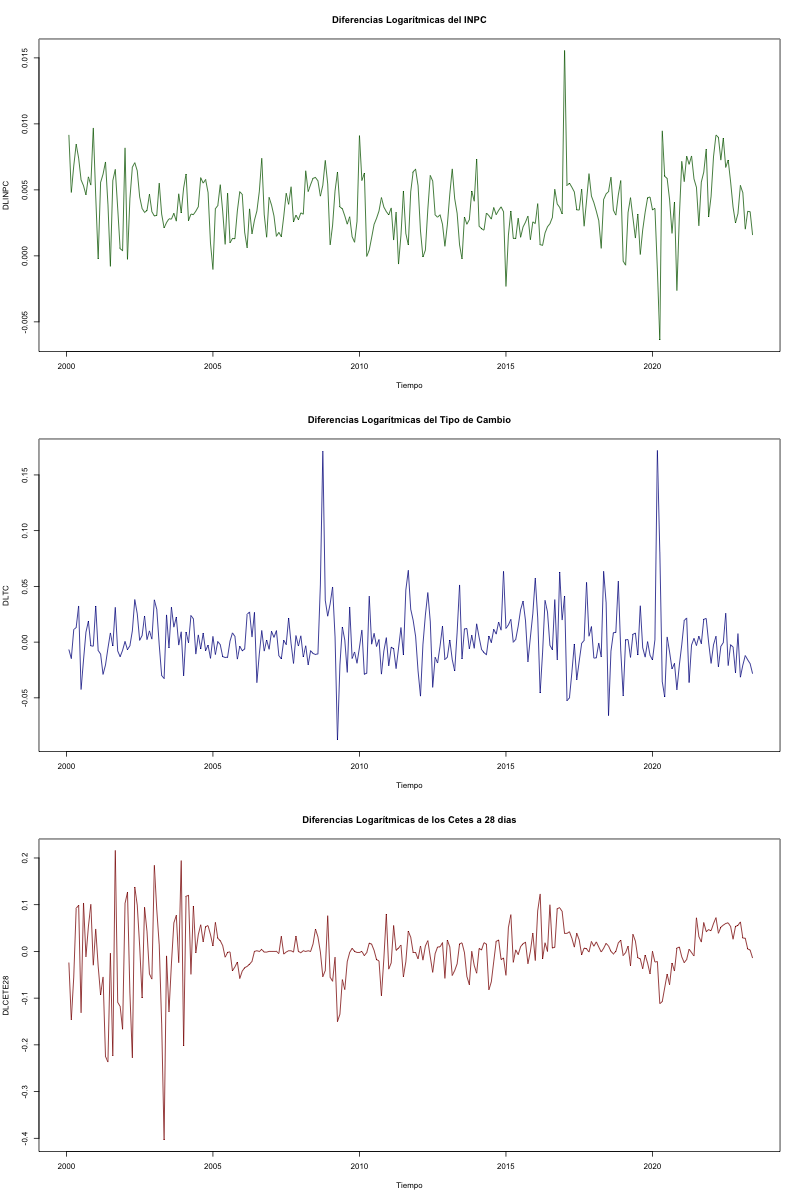
\includegraphics[width = 1.0 \textwidth]{DLGranger}
    \caption{Series en diferencias logarítmicas dadas por las siguientes expresiones: $DLINPC_t = ln(DLINPC_t) - ln(DLINPC_{t-1})$, $DLTC_t = ln(TC_t) - ln(TC_{t-1})$ y $DLCETE28_t = ln(CETE28_t) - ln(CETE28_{t-1})$.}
  \label{DLGranger}
\end{figure}

Por simplicidad, en el Cuadro (\ref{Granger_01}) se muestra el resultado
de aplicar el test de Granger a diferentes especificaciones, con rezagos
4, 8, 12 y 16, sólo para la serie de Tipo de Cambio en diferencias
logarítmicas. En cada una de las pruebas se compara el modelo
considerado como regresor a la variable que es candidata de causar,
respecto del modelo si considerar a dicha variable.

\begin{table}
\centering
\begin{tabular}{| c | c | c | c |}
\hline
    Rezagos & Estadiística F & Probabilidad ($>$F) & Significancia \\
\hline
    4 & 3.2621 & 0.01265 & * \\
    8 & 1.9079 & 0.06030 &  \\
    12 & 2.2577 & 0.01067 & * \\
    16 & 1.6735 & 0.05495 & * \\
\hline
    \multicolumn{4}{ l }{Notas: *** significancia al 0.001\%, ** significancia al 0.01\% y } \\
    \multicolumn{4}{ l }{* significancia 0.05\%} \\
\end{tabular}
    \caption{Prueba de si $DLINPC_t$ Granger causa a $DLTC_t$.}
    
\end{table}

De acuerdo con el Cuadro (\ref{Granger_01}), podemos concluir que existe
información estadísticamente significativa para concluir que la
inflación causa a la tasa de depreciación cambiaria, ambas medidas como
las diferencias logaritmicas. El resto de los resultados para las otras
combinaciones de causalidad se encuentran en el Scrip llamado Clase 13
ubicado en el repositorio de GitHub.

\subsection{Definición y representación del Sistema o Modelo
VAR(p)}\label{definiciuxf3n-y-representaciuxf3n-del-sistema-o-modelo-varp}

En esta sección ampliaremos la discusión planteada en el apartado
anterior. En el sentido de que en la sección pasada nuestra discusión se
limito al análisis de causalidad entre dos variables a la vez, que si
bien es posible extenderlo a más variables es un procedimiento limitado
a casos particulares por las siguientes razones.

El procediento de causalidad de Granger supone que es posible
identificar un sistema de ecuaciones que debe conformarse una vez que se
ha identificado el sentido de la causalidad. Así, el proceso anterior
necesita del conocimiento previo de las relaciones que existen entre las
varibles.

Adicionalmente, no resuleve el problema más general qué esta relacionado
con cómo identificar la causalidad cuando se tienen múltiples variables
con múltiples sentidos de causalidad. En esta sección analizaremos una
mejor aproximación al probelma de cómo identificar la causalidad
múltiple. Por lo tanto, como mécanismo para solucionar el problema
planteado, analizaremos el caso de un Sistema o Modelo de Vectores
Autoregresivos conocido como VAR.

El primer supuesto del que partiremos es que existe algún grado de
endogenidad entre las variables considerdas en el análisis.
Adicionalmente, el segundo supuesto que estableceremos es que requerimos
que las variables que tengamos consideradas sean estacionarias.

Por lo anterior diremos que un VAR es un procedimiento que sigue fundado
en el supuesto de que las variables consideredas son estacionarias, sin
que hasta el momento hallamos podido establecer un mécanismo de
detección de dicha estacionariedad. Así, hasta este momento del curso
hemos pasado de modelo univariados a modelo múltivariados, pero no hemos
podido dejar de asumir que las series son estacionarias.

Ahora bien, iniciaremos con el establecimiento de la representación del
proceso. Digamos que tenemos un proceso estocástico \(\mathbf{X}\)
estacionario de dimensión \(k\). De esta forma la expresión reducida del
modelo o el proceso \(VAR(p)\) estará dado por: \[
    \mathbf{X}_t = \mathbf{\delta} + A_1 \mathbf{X}_{t-1} + A_2 \mathbf{X}_{t-2} + \ldots + A_p \mathbf{X}_{t-p} + \mathbf{U}_{t}
    \label{VAR_p}
\]

Donde cada uno de las \(A_i\), \(i = 1, 2, \ldots, p\), son matrices
cuadradas de dimensión \(k\) y \(\mathbf{U}_t\) representa un vector de
dimensión \(k \times 1\) con los residuales en el momento del tiempo
\(t\) que son un proceso pueramente aleatorio. También se incorpora un
vector de términos constantes denominado como \(\mathbf{\delta}\), el
cual es de dimensión \(k \times 1\).

Así, la ecuación (\ref{VAR_p}) supone la siguiente estructura de
vectores: \begin{equation*}
    \mathbf{X}_t = 
    \begin{bmatrix}
    X_{1t} \\ X_{2t} \\ \vdots \\ X_{kt}
    \end{bmatrix}
\end{equation*}

Para cualquier \(i = 1, 2, \ldots, p\): \begin{equation*}
    \mathbf{X}_{t-i} = 
    \begin{bmatrix}
    X_{1t-i} \\ X_{2t-i} \\ \vdots \\ X_{kt-i}
    \end{bmatrix}
\end{equation*}

\begin{equation*}
    \mathbf{\delta} = 
    \begin{bmatrix}
    \delta_{1} \\ \delta_{2} \\ \vdots \\ \delta_{k}
    \end{bmatrix}
\end{equation*}

También, la ecuación (\ref{VAR_p}) supone que cada matriz \(A_i\),
\(i = 1, 2, \ldots, p\), esta definida de la siguiente forma:
\begin{equation*}
    \mathbf{A}_i = 
    \begin{bmatrix}
    a^{(i)}_{11} & a^{(i)}_{12} & \ldots & a^{(i)}_{1k} \\ a^{(i)}_{21} & a^{(i)}_{22} & \ldots & a^{(i)}_{2k} \\ \vdots & \vdots & \ddots & \vdots \\ a^{(i)}_{k1} & a^{(i)}_{k2} & \ldots & a^{(i)}_{kk}
    \end{bmatrix}
\end{equation*}

Retomando la ecuación (\ref{VAR_p}) y considerando que podemos ocupar el
operador rezago \(L^j\) de forma analóga al caso del modelo \(AR(p)\),
pero aplicado a un vector, tenemos las siguientes ecuaciones:
\begin{eqnarray}
    \mathbf{X}_t - A_1 \mathbf{X}_{t-1} - A_2 \mathbf{X}_{t-2} - \ldots - A_p \mathbf{X}_{t-p} & = & \mathbf{\delta} + \mathbf{U}_{t} \nonumber \\
    \mathbf{X}_t - A_1 L \mathbf{X}_{t} - A_2 L^2 \mathbf{X}_{t} - \ldots - A_p L^p \mathbf{X}_{t-p} & = & \mathbf{\delta} + \mathbf{U}_{t} \nonumber \\
    (I_k - A_1 L - A_2 L^2 - \ldots - A_p L^p) \mathbf{X}_t & = & \mathbf{\delta} + \mathbf{U}_{t} \nonumber \\
    \mathbf{A}(L) \mathbf{X}_t & = & \mathbf{\delta} + \mathbf{U}_{t}
    \label{VAR_Corto}
\end{eqnarray}

Adicionalmente, requeriremos que dado que \(\mathbf{U}_t\) es un proceso
pueramente aleatorio, este debe cumplir con las siguientes condiciones:

\begin{enumerate}
    \item El valor esperado del término de erros es cero:
    $$
        \mathbb{E}[\mathbf{U}_t] = 0
    $$

    \item Existe una matriz de varianzas y covarianzas entre los términos de error contemporáneos dada por:
    \begin{eqnarray}
        \mathbb{E}[\mathbf{U}_t \mathbf{U}_t'] 
        & = &
        \mathbb{E} \left[
        \begin{bmatrix}
        U^{(t)}_{1} \\ U^{(t)}_{2} \\ \vdots \\ U^{(t)}_{k}
        \end{bmatrix}
        \begin{bmatrix}
        U^{(t)}_{1} & U^{(t)}_{2} & \ldots & U^{(t)}_{k}
        \end{bmatrix}
        \right] \nonumber \\
        & = & \mathbb{E}
        \begin{bmatrix}
        U^{(t)}_{1} U^{(t)}_{1} & U^{(t)}_{1} U^{(t)}_{2} & \ldots & U^{(t)}_{1} U^{(t)}_{k} \\
        U^{(t)}_{2} U^{(t)}_{1} & U^{(t)}_{2} U^{(t)}_{2} & \ldots & U^{(t)}_{2} U^{(t)}_{k} \\
        \vdots & \vdots & \ldots & \vdots \\
        U^{(t)}_{k} U^{(t)}_{1} & U^{(t)}_{k} U^{(t)}_{2} & \ldots & U^{(t)}_{k} U^{(t)}_{k}
        \end{bmatrix} \nonumber \\
        & = & \begin{bmatrix}
        \sigma^2_1 & \rho_{12} & \ldots & \rho_{1k} \\
        \rho_{21} & \sigma^2_2 & \ldots & \rho_{2k} \\
        \vdots & \vdots & \ldots & \vdots \\
        \rho_{k1} & \rho_{k2} & \ldots & \sigma^2_k
        \end{bmatrix} \nonumber \\
        & = & \mathbf{\Sigma}_{UU}
        \label{Sigma_VAR}
    \end{eqnarray} 

    \item La matriz de varianzas y covarianzas no comtemporáneas es nula. Es decir, que para todo $t \neq s$:
    \begin{eqnarray}
        \mathbb{E} [\mathbf{U}_t \mathbf{U}_s'] 
        & = &
        \mathbb{E} \left[
        \begin{bmatrix}
        U^{(t)}_{1} \\ U^{(t)}_{2} \\ \vdots \\ U^{(t)}_{k}
        \end{bmatrix}
        \begin{bmatrix}
        U^{(s)}_{1} & U^{(s)}_{2} & \ldots & U^{(s)}_{k}
        \end{bmatrix}
        \right] \nonumber \\
        & =  & \mathbb{E}
        \begin{bmatrix}
        U^{(t)}_{1} U^{(s)}_{1} & U^{(t)}_{1} U^{(s)}_{2} & \ldots & U^{(t)}_{1} U^{(s)}_{k} \\
        U^{(t)}_{2} U^{(s)}_{1} & U^{(t)}_{2} U^{(s)}_{2} & \ldots & U^{(t)}_{2} U^{(s)}_{k} \\
        \vdots & \vdots & \ldots & \vdots \\
        U^{(t)}_{k} U^{(s)}_{1} & U^{(t)}_{k} U^{(s)}_{2} & \ldots & U^{(t)}_{k} U^{(s)}_{k}
        \end{bmatrix} \nonumber \\
        & = & \mathbf{0}
        \label{Rho_VAR}
    \end{eqnarray}
\end{enumerate}

Las ecuaciones (\ref{Sigma_VAR}) y (\ref{Rho_VAR}) significan que los
residuales \(\mathbf{U}_t\) pueden estar correlacionados entre ellos
solo en el caso de que la información sea contemporánea, pero no tienen
información en común entre residuales de otros periodos.

Al igual que en el caso del modelo o especificación \(AR(p)\) en la
especificación del modelo \(VAR(p)\) existen condiciones de estabilidad.
Dichas condiciones están dadas por lo siguiente, definamos el siguiente
polinomio que resulta de tomar la matriz \(\mathbf{A}(L)\) en la
ecuación (\ref{VAR_Corto}): \[
    Det[I_t - A_1 z - A_2 z^2 - \ldots - A_p z^p] \neq 0
\]

Donde las raíces del polinomio cumplen que \(|z| \leq 1\), es decir, se
ubican dentro del circulo unitario.

La ecuación (\ref{VAR_Corto}) puede ser rexpresada en una forma similar
al un proceso de MA. Al respecto, de forma similar a la siguiente
ecuación podemos construir un modelo \(VARMA(p,q)\), el cual no
estudiamos es este curso.

Reromando el primer planteamiento, podemos escribir: \begin{eqnarray}
    \mathbf{X}_t & = & \mathbf{A}^{-1}(L) \delta + \mathbf{A}^{-1}(L) \mathbf{U}_t \nonumber \\
    & = & \mu + \beta(L) \mathbf{U}_t
    \label{VARMA_q}
\end{eqnarray}

Por el lado de las matrices que representan la autocovarianza, estás
resultan de resolver lo siguiente: \[
    \Gamma_X(\tau) = E[(\mathbf{X}_t - \mu)(\mathbf{X}_{t-\tau} - \mu)'] 
\]

Ahora, sin pérdida de generalidad digamos que la especificación VAR(p)
en la ecuación (\ref{VAR_p}) no tiene constante, por lo que
\(\delta = 0\), lo que implica que \(\mu = 0\). De esta forma las
matrices de autocovarianza resultan de: \begin{eqnarray*}
    \Gamma_X(\tau) & = & E[(\mathbf{X}_t)(\mathbf{X}_{t-\tau})'] \\
    & = & A_1 E[(\mathbf{X}_{t-1})(\mathbf{X}_{t-\tau})'] + A_2 E[(\mathbf{X}_{t-2})(\mathbf{X}_{t-\tau})'] \\
    &   & + \ldots + A_p E[(\mathbf{X}_{t-p})(\mathbf{X}_{t-\tau})'] + E[(\mathbf{U}_t(\mathbf{X}_{t-\tau})']
\end{eqnarray*}

Finalmente, al igual que en el caso \(AR(p)\) requerimos de una métrica
que nos permita determinar el número de rezagos óptimo \(p\) en el
\(VAR(p)\). Así, establecemos criterios de información similares a los
del \(AR(p)\) dados por:

\begin{enumerate}
    \item Final Prediction Error (FPE):
        $$
        FPE(p) = \left[ \frac{T + kp + 1}{T - kp - 1} \right]^k |\mathbf{\Sigma}_{\hat{U}\hat{U}}(p)|
        $$
    
    \item Akaike Criterion (AIC):
        $$
        AIC(p) = ln|\mathbf{\Sigma}_{\hat{U}\hat{U}}(p)| + (k + p k^2) \frac{2}{T}
        $$
    
    \item Hannan - Quinn Criterion (HQ):
        $$
        HQ(p) = ln|\mathbf{\Sigma}_{\hat{U}\hat{U}}(p)| + (k + p k^2) \frac{2ln(ln(2))}{T}
        $$
    
    \item Schwartz Criterion (SC):
        $$
        SC(p) = ln|\mathbf{\Sigma}_{\hat{U}\hat{U}}(p)| + (k + p k^2) \frac{ln(T)}{T}
        $$
        
        Donde la matriz de varianzas y covarianzas contemporáneas estará dada por:
        \begin{equation*}
            \mathbf{\Sigma}_{\hat{U}\hat{U}}(p) = \mathbb{E} \left[
            \begin{bmatrix}
            U^{(t)}_{1} \\ U^{(t)}_{2} \\ \vdots \\ U^{(t)}_{k}
            \end{bmatrix}
            \begin{bmatrix}
            U^{(t)}_{1} & U^{(t)}_{2} & \ldots & U^{(t)}_{k}
            \end{bmatrix}
            \right]
        \end{equation*}
\end{enumerate}

Ahora veámos un ejemplo de estimación de \(VAR(p)\). Para el ejemplo
utilizaremos las series de INPC, Tipo de CAmbio, rendimiento de los
Cetes a 28 días, el IGAE y el Índice de Producción Industrial de los
Estados Unidos, todas desestacionalizadas y para el período de enero de
2000 a julio de 2019. Dado que el supuesto estacionariedad sigue
presente en nuestro análisis, emplearemos cada una de las series en su
versión de diferencias logaritmicas. La Figura (\ref{VAR_DLSeries})
muestra las series referidas.

\begin{figure}
  \centering
    \includegraphics[width = 1.0 \textwidth]{VAR_DLSeries}
  \caption{Series en diferencias logarítmicas, enero de 2000 a julio de 201p}
  \label{VAR_DLSeries}
\end{figure}

Dicho lo anterior, a continuación mostraremos la tabla que resume el
valor de los distintos criterios de información una especificación de un
\(VAR(p)\) con constante. Notése que es posible especificar un
\(VAR(p)\) con tendencia, caso que no aplica hasta este momento, ya que
nuestro análisis de estacionariedad es claro respecto a la media
constante (más adelante relajaremos este supuesto), lo cual elimina la
poisiblidad de incluir una tendencia.

En el Cuadro (\ref{Select_VAR}) reportamos los resultados de aplicar una
prueba de criterios de información para diferentes valores de reagos.
Del cual se concluye que el número óptimo de residuales es 2 (según el
crietrio AIC y el FPE) y 1 (según el criterio HQ y el SC). Recordemos
que es común que el criterio AIC siempre reporte el mayor valor de
rezagos, por lo que es una buena práctica utilizarlo como referente
principal.

\begin{table}
\centering
\begin{tabular}{| c | c | c | c | c |}
\hline
    Rezagos & AIC & HQ & SC & FPE \\
\hline
    1 & -4.636412e+01 & -4.617847e+01 & -4.590430e+01 & 7.317262e-21 \\
    2 & -4.639541e+01 & -4.605506e+01 & -4.555241e+01 & 7.094216e-21 \\
    3 & -4.635305e+01 & -4.585799e+01 & -4.512686e+01 & 7.407479e-21 \\
    \vdots & \vdots & \vdots & \vdots & \vdots \\
\hline
    \multicolumn{5}{ l }{Nota: Se reporta el valor de los criterios de información.} \\
\end{tabular}
\caption{Criterios de información para diferentes especificaciones de modelos VAR(p) con término constante de la series $DLINPC_t$, $DLTC_t$, $DLCETE28_t$, $DLIGAE_t$ y $DLIPI_t$.}

\end{table}

De esta forma, justificamos la estimación de un \(VAR(2)\). Los
resultados del mismo se repotartan en los siguientes cuadros, en los que
se reporta el resultado de una de las ecuaciones. Los resultados
restantes se encuentran en el Scrip Clase 14 que se encuentra en
repositorio de GitHub. Primero mostraremos los resutlados de las raíces
del polinomio caracteristico en el Cuadro (\ref{Roots_VAR}), seguido de
un cuadro para la ecuación del IGAE en el Cuadro (\ref{IGAE_VAR})(por
simplicidad se omiten las otras cuatro ecuaciones del VAR(2)), y del
Cuadro (\ref{Sigma_VARp}) con la matriz
\(\mathbf{\Sigma}_{\hat{U}\hat{U}}\) estimada del VAR.

\begin{table}
\centering
\begin{tabular}{| c | c | c | c | c |}
\hline
    0.7452 & 0.4403 & 0.4403 & 0.3503 & 0.3503 \\
    \hline
    0.3342 & 0.3342 & 0.3339 & 0.3339 & 0.06951 \\
\hline
\end{tabular}
\caption{Raíces del polinomio característico de un VAR(2).}

\end{table}

\begin{table}
\centering
\begin{tabular}{| c | c | c | c | c |}
\hline
    Variable & Coeficiente & Error Est. & Estad. t & Prob.($>$ t) \\
\hline
    $DLINPC_{t-1}$ & -0.2584978 & 0.1658396 & -1.559 & 0.120493 \\
    $DLTC_{t-1}$ & 0.0022016 & 0.0152876 & 0.144 & 0.885620 \\
    $DLCETE28_{t-1}$ & 0.0009547 & 0.0049115 & 0.194 & 0.846054 \\
    $DLIGAE_{t-1}$ & -0.2351453 & 0.0699797 & -3.360 & 0.000917 *** \\
    $DLIPI_{t-1}$ & 0.2442406 & 0.0600502 & 4.067 & 6.62e-05 *** \\
    $DLINPC_{t-2}$ & -0.0775039 & 0.1694809 & -0.457 & 0.647904 \\
    $DLTC_{t-2}$ & -0.0413316 & 0.0144650 & -2.857 & 0.004680 ** \\
    $DLCETE28_{t-2}$ & 0.0005341 & 0.0048058 & 0.111 & 0.911612 \\
    $DLIGAE_{t-2}$ & -0.0646890 & 0.0693711 & -0.933 & 0.352092 \\ 
    $DLIPI_{t-2}$ & 0.1796286 & 0.0620861 & 2.893 & 0.004195 ** \\
    $\delta_4$ & 0.0030377 & 0.0008077 & 3.761 & 0.000217 *** \\
\hline
    \multicolumn{5}{ l }{Nota: *** significancia al 0.001\%, ** significancia al 0.01\%,} \\
    \multicolumn{5}{ l }{significancia 0.05\%} \\
\end{tabular}
\caption{Criterios de información para diferentes especificaciones de modelos VAR(p) con término constante de la series $DLINPC_t$, $DLTC_t$, $DLCETE28_t$, $DLIGAE_t$ y $DLIPI_t$.}

\end{table}

\begin{table}
\centering
\begin{tabular}{| c | c  c  c  c  c |}
\hline
     & $DLINPC_t$ & $DLTC_t$ & $DLCE28_t$ & $DLIGAE_t$ & $DLIGAE_t$ \\ \hline
    $DLINPC_t$ & 3.95e-06 & 3.19e-06 & -1.83e-06 & -5.29-07 & 1.34e-06 \\
    $DLTC_t$ & 3.19e-06 & 5.04e-04 & 4.27e-04 & 9.81e-06 & 1.61e-05 \\
    $DLCE28_t$ & -1.83e-06 & 4.27e-04 & 4.63e-03 & 1.26e-05 & 2.76e-05 \\
    $DLIGAE_t$ & -5.29e-07 & 9.81e-06 & 1.26e-05 & 2.43e-05 & 8.75e-06 \\
    $DLIGAE_t$ & 1.34e-06 & 1.61e-05 & 2.76e-05 & 8.75e-06 & 3.13e-05 \\
\hline
\end{tabular}
\caption{Matriz $\mathbf{\Sigma}_{\hat{U}\hat{U}}$ estimada del VAR(2).}

\end{table}

Finalmente, en el Cuadro (\ref{Diagnos_VAR}) reportamos las pruebas de
diagnóstico del VAR(2). Incluímos las pruebas de normalidad,
autocorrelación parcial y de heterocedásticidad.

\begin{table}
\centering
\begin{tabular}{| c | c | c | c |}
\hline
    Estadística (rezagos) & Coeficiente & p-value & Conclusión \\ 
\hline
    Correlación Serial ($\chi^2 (2)$) & 59.436 & 0.1696 & Existe auto- \\
     &  &  & correlación serial \\
    Correlación Serial ($\chi^2 (4)$) & 127.17 & 0.03461 & No existe auto- \\
     &  &  & correlación serial \\
    Correlación Serial ($\chi^2 (6)$) & 183.14 & 0.03393 & No existe auto- \\
     &  &  & correlación serial \\
    Normalidad - JB ($\chi^2$) & 2335 & 0.0000 & Los residuales \\
     &  &  & no son normales \\
    ARCH ($\chi^2 (2)$) & 691.58 & 0.0000 & Los residuales no \\
     &  &  & son homocedásticos \\
\hline
\end{tabular}
\caption{Pruebas de diagnóstico sobre los residuales del VAR(2).}

\end{table}

\subsection{Análisis de
Impulso-Respuesta}\label{anuxe1lisis-de-impulso-respuesta}

Una de las grandes ventajas que aporta el análisis de los modelos VAR es
el análisis de Impulso-Respuesta. Dicho análisis busca cuantificar el
efecto que tiene en \(\mathbf{X}_t\) una innovación o cambio en los
residuales de cualquiera de las variables en un momento definido.
Partamos dela ecuación (\ref{VARMA_q}) de forma que tenemos:
\begin{eqnarray}
    \mathbf{X}_t & = & \mathbf{A}^{-1}(L) \delta + \mathbf{A}^{-1}(L) \mathbf{U}_t \nonumber \\
    & = & \mu + \mathbf{B}(L) \mathbf{U}_t \nonumber \\
    & = & \mu + \Psi_0 \mathbf{U}_t + \Psi_1 \mathbf{U}_{t-1} + \Psi_2 \mathbf{U}_{t-2} + \Psi_3 \mathbf{U}_{t-3} + \ldots
\end{eqnarray}

Donde \(\Psi_0 = I\) y cada una de las \(\Psi_i = - \mathbf{B}_i\),
\(i = 1, 2, \ldots\). De esta forma se verifica el efecto que tiene en
\(\mathbf{X}_t\) cada las innovaciones pasadas. Por lo que el análisis
de Impulso-Respuesta cuantifica el efecto de cada una de esas matrices
en las que hemos descompuesto a \(\mathbf{B}(L)\).

Retomando el modelo \(VAR(2)\) anteriormente estimado, en el Cuadro
(\ref{IR_VAR_TC}) reportamos las gráficas de Impulso-respuesta de la
serie \(DLTC_t\) ante cambios en los residuales del resto de las series
y de la propia serie.

\begin{table}
\centering
\begin{tabular}{ c c }
\begin{subfigure}\centering\includegraphics[width = 0.45\columnwidth]{IR_DLTC_1}\end{subfigure} & 
\begin{subfigure}\centering\includegraphics[width = 0.45\columnwidth]{IR_DLTC_2}\end{subfigure} \\
\newline
\begin{subfigure}\centering\includegraphics[width = 0.45\columnwidth]{IR_DLTC_3}\end{subfigure} & 
\begin{subfigure}\centering\includegraphics[width = 0.45\columnwidth]{IR_DLTC_4}\end{subfigure} \\
\newline
\begin{subfigure}\centering\includegraphics[width = 0.45\columnwidth]{IR_DLTC_5}\end{subfigure} & 
%\begin{subfigure}\centering\includegraphics[width=0.45\columnwidth]{IR_DLTC_6}\end{subfigure} \\
\end{tabular}
\caption{Gráficas de Impulso-respuesta de la serie $DLTC_t$ ante cambios en los residuales del resto de las series y de la propia serie.}

\end{table}

Los resultados muestran que la respuesta de \(DLTC_t\) ante impulsos en
los términos de error fue estadísticamente significativo sólo para
alguunos de los casos y en periodos cortos de tiempo. El resto de los
resultados de Impulso-Respuesta se encuentra en el Scrip llamado Clase
15 que se ubica en el repositorio de GitHub.


\printbibliography


\end{document}
